\section{Enjeu de l'informatique décisionnelle}
Nous vivons dans un monde ou chaque action, chaque opération génère des données Cette assertion s'applique évidement au monde de l'entreprise, ou l’activité est plus que jamais organisée et formalisée sous formes de processus.
A chaque étape du processus métier, un quotta de donnée est généré de façon à tracer l’activité de l’entreprise. Ces données peuvent être de plusieurs types, références, fournisseurs ou encore analytiques.\\
Malheureusement, ce rapport à la donnée amène la constitution de gigantesque “DataWarehouses”, ou entrepôts de données possédant une telle complexité et multiplicité qu’ils en deviennent inexploitables. Sans interprétation, traitement et exploitation préalable il devient impossible de déduire quelque chose de ces entrepôts de données.\\
Le besoin est donc clair, il faut “donner” de la visibilité à ces entrepôts de données. Ainsi, par la définitions de différents tableau d’indicateurs synthétiques et pertinents, il deviens facile d’exploiter les données collectées. Ceci est particulièrement destiné au public de décideurs, non informaticiens... \\
Plus loin encore, certains procédés permettent de générée des données à partir d’autres données de masses. En effet en isolant des tendances, des modèles d’actions entre les différentes entités, nous sommes en mesure d'obtenir de nouvelles informations insoupçonnées.\\
C’est ici qu'interviennent les solutions de business intelligence, ou informatique décisionnelle. Par ce terme, il est désigné l'ensemble des outils ou méthodes appliquées à la donnée, depuis sa collecte, jusqu’à la définition de “tableau de bords” à destination des décideurs.
Ainsi nous pouvons isoler les étapes suivantes :
\begin{itemize}
\item[•]Collecte : Cette phase englobe les étapes d'extraction des données, de traitement et enfin chargée dans l'entrepôt de données. Elles est plus souvent déléguée à des outils type ETL fournis par des grands acteurs du domaine.
\item[•]Intégration : Il ne suffit pas de charger les données pour les rendre exploitables. Ainsi tout un procédé de nettoyage, synchronisation avec les données actuelles, et enfin de certification. Sans cette étape, la pérennité de l'entrepôt de données serait mise en question par un grand nombre de données incorrectes / corrompues et surtout non exploitables.
\item[•]Distribution : Du fait de la taille de l'entrepôt de données, il est impossible de traiter la globalité des données, ainsi, le regroupement des données et la distribution en sous ensemble cohérents d’un point de vue opérationnel, (ie un regroupement par secteur...)  est nécessaire, de façon à optimiser les temps de traitements des diverses applications exploitant ces données.
\item[•]Présentation : Sous la forme d’indicateurs concrets, voire de tableaux de bord classiques, les données sont exprimées de manière à ce que n’importe quel utilisateur final puisse les comprendre et en tenir compte dans les décisions de la façon la plus complète possible.
\item[•]Administration :  Des fonctionnalités d’administration du DataWarehouse, de son alimentation, une gestion des compte / application utilisatrices de ces données, impliquant un contrôle d’accès, de répartition de la charge et autres implications importantes délégués au contrôle des systèmes de données de grande envergure.
\end{itemize}

\begin{figure}[H]
\begin{center}
  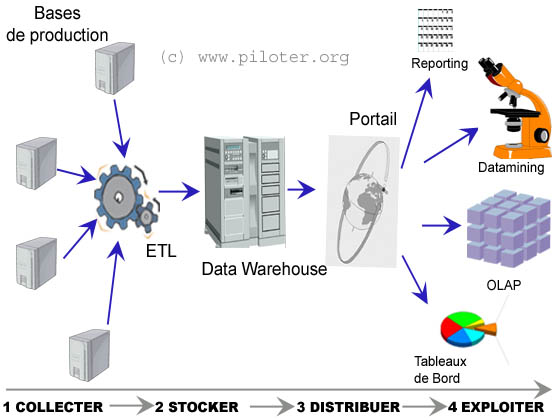
\includegraphics[scale= 0.5]{Enjeu.jpg}
  \caption{Les 4 phases du processus de Business Intelligence : de la donnée à l'information.}
\end{center}  
\end{figure}
